\begin{figure}[htbp]
			\centering
			\resizebox{\textwidth}{!}{%
				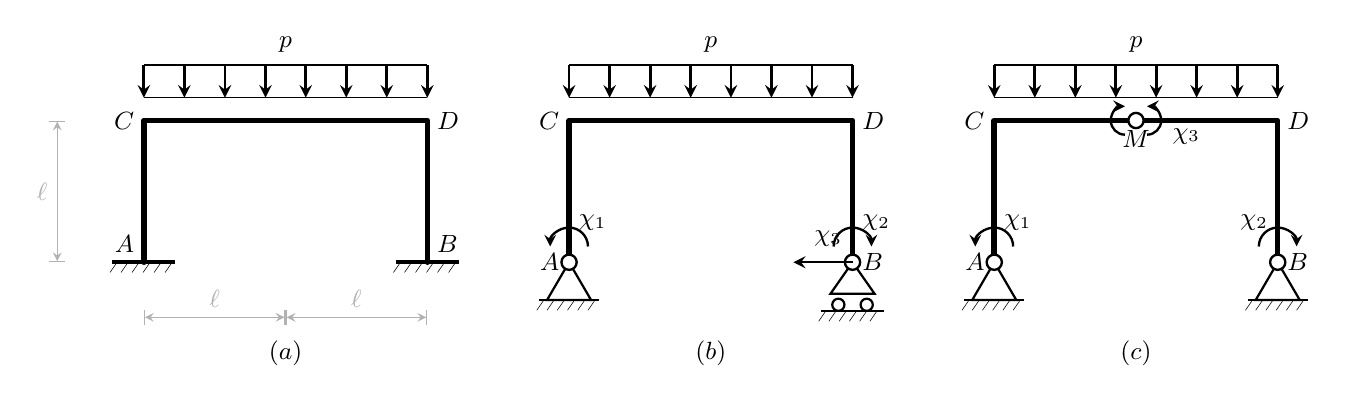
\begin{tikzpicture}[
					trave/.style={line width=2.0pt, line cap=round, line join=round, black},
					terra/.style={line width=0.8pt, black},
					carico/.style={->, >=stealth, line width=1.0pt, black},
					nodoV/.style={circle, fill=white, draw=black,
						inner sep=0pt, minimum size=5.5pt, line width=0.85pt},
					quota/.style={|<->|, >=stealth, thin, gray!60},
					]  
					
					\def\L{1.80}   % ℓ in cm
					\def\SEP{5.40} % separazione tra i pannelli
					\def\Lc{2.00}   % = \L + 0.20
					
					%%═══ PANNELLO (a) — portale doppiamente incastrato ══════════════════════
					\begin{scope}[xshift=0cm]
						%% Travi
						\draw[trave](0,0)--(0,\L)--(2*\L,\L)--(2*\L,0);
						%% Incastro in A
						\draw[terra,line width=1.4pt](-0.40,0)--(0.40,0);
						\foreach \x in {-0.34,-0.20,-0.06,0.08,0.22,0.36}
						\draw[very thin](\x,0)--++(-0.09,-0.13);
						%% Incastro in B
						\draw[terra,line width=1.4pt]({2*\L-0.40},0)--({2*\L+0.40},0);
						\foreach \x in {-0.34,-0.20,-0.06,0.08,0.22,0.36}
						\draw[very thin]({2*\L+\x},0)--++(-0.09,-0.13);
						%% Carico uniforme p
						\foreach \t in {0.0,0.143,0.286,0.429,0.571,0.714,0.857,1.00}{
							\draw[carico]({2*\L*\t},{\Lc+0.50})--({2*\L*\t},{\Lc+0.09});}
						\draw[black,line width=0.65pt](0,{\Lc+0.50})--(2*\L,{\Lc+0.50});
						\draw[black,line width=0.40pt](0,{\Lc+0.09})--(2*\L,{\Lc+0.09});
						\node[above,font=\small]at(\L,{\Lc+0.54}){$p$};
						%% Etichette nodi
						\node[above left,font=\small]at(0,0){$A$};
						\node[above right,font=\small]at(2*\L,0){$B$};
						\node[left,font=\small]at(0,\L){$C$};
						\node[right,font=\small]at(2*\L,\L){$D$};
						%% Quote dimensionali
						\draw[quota](-1.10,0)--(-1.10,\L)node[midway,left,font=\small]{$\ell$};
						\draw[quota](0,-0.70)--(\L,-0.70)node[midway,above,font=\small]{$\ell$};
						\draw[quota](\L,-0.70)--(2*\L,-0.70)node[midway,above,font=\small]{$\ell$};
						\node[font=\small]at(\L,-1.15){$(a)$};
					\end{scope}
					
					%%═══ PANNELLO (b) — sistema principale «portale appoggiato» ═════════════
					\begin{scope}[xshift=\SEP cm]
						%% Travi
						\draw[trave](0,0)--(0,\L)--(2*\L,\L)--(2*\L,0);
						%% Cerniera in A
						\draw[terra](0,0)--(-0.28,-0.48)--(0.28,-0.48)--cycle;
						\draw[terra](-0.38,-0.48)--(0.38,-0.48);
						\foreach \x in {-0.32,-0.19,-0.06,0.07,0.20,0.33}
						\draw[very thin](\x,-0.48)--++(-0.09,-0.13);
						\node[nodoV]at(0,0){};
						%% Carrello con piano di scorrimento orizzontale in B
						\draw[terra](2*\L,0)--(2*\L-0.28,-0.40)--(2*\L+0.28,-0.40)--cycle;
						\draw[terra](2*\L-0.18,-0.54)circle(2.2pt);
						\draw[terra](2*\L+0.18,-0.54)circle(2.2pt);
						\draw[terra]({2*\L-0.40},-0.62)--({2*\L+0.40},-0.62);
						\foreach \x in {-0.34,-0.21,-0.08,0.05,0.18,0.31}
						\draw[very thin]({2*\L+\x},-0.62)--++(-0.09,-0.13);
						\node[nodoV]at(2*\L,0){};
						%% Carico uniforme p
						\foreach \t in {0.0,0.143,0.286,0.429,0.571,0.714,0.857,1.00}{
							\draw[carico]({2*\L*\t},{\Lc+0.50})--({2*\L*\t},{\Lc+0.09});}
						\draw[black,line width=0.65pt](0,{\Lc+0.50})--(2*\L,{\Lc+0.50});
						\draw[black,line width=0.40pt](0,{\Lc+0.09})--(2*\L,{\Lc+0.09});
						\node[above,font=\small]at(\L,{\Lc+0.54}){$p$};
						%% Etichette nodi
						\node[left,font=\small]at(0,0){$A$};
						\node[right,font=\small]at(2*\L,0){$B$};
						\node[left,font=\small]at(0,\L){$C$};
						\node[right,font=\small]at(2*\L,\L){$D$};
						%% χ₁ — coppia antioraria in A: semiarco che attraversa la colonna,
						%%       convessità verso l'alto; centro (0, 0.20), raggio 0.24
						\draw[->,>=stealth,line width=0.85pt](0.24,0.20)arc(0:180:0.24);
						\node[right,font=\small]at(0,0.50){$\chi_1$};
						%% χ₂ — coppia oraria in B: semiarco speculare a χ₁,
						%%       centro (2ℓ, 0.20), raggio 0.24
						\draw[->,>=stealth,line width=0.85pt]({2*\L-0.24},0.20)arc(180:0:0.24);
						\node[right,font=\small]at(2*\L,0.50){$\chi_2$};
						%% χ₃ — reazione orizzontale rimossa: coda in B, punta verso A
						\draw[->,>=stealth,line width=0.90pt](2*\L,0)--({2*\L-0.75},0);
						\node[left=0.3,font=\small]at(2*\L,0.30){$\chi_3$};
						\node[font=\small]at(\L,-1.15){$(b)$};
					\end{scope}
					
					%%═══ PANNELLO (c) — sistema principale «portale a tre cerniere» ══════════
					\begin{scope}[xshift={2*\SEP cm}]
						%% Travi
						\draw[trave](0,0)--(0,\L)--(2*\L,\L)--(2*\L,0);
						%% Cerniera in A
						\draw[terra](0,0)--(-0.28,-0.48)--(0.28,-0.48)--cycle;
						\draw[terra](-0.38,-0.48)--(0.38,-0.48);
						\foreach \x in {-0.32,-0.19,-0.06,0.07,0.20,0.33}
						\draw[very thin](\x,-0.48)--++(-0.09,-0.13);
						\node[nodoV]at(0,0){};
						%% Cerniera in B
						\draw[terra](2*\L,0)--(2*\L-0.28,-0.48)--(2*\L+0.28,-0.48)--cycle;
						\draw[terra]({2*\L-0.38},-0.48)--({2*\L+0.38},-0.48);
						\foreach \x in {-0.32,-0.19,-0.06,0.07,0.20,0.33}
						\draw[very thin]({2*\L+\x},-0.48)--++(-0.09,-0.13);
						\node[nodoV]at(2*\L,0){};
						%% Cerniera interna in M (mezzeria del traverso)
						\node[nodoV]at(\L,\L){};
						%% Carico uniforme p
						\foreach \t in {0.0,0.143,0.286,0.429,0.571,0.714,0.857,1.00}{
							\draw[carico]({2*\L*\t},{\Lc+0.50})--({2*\L*\t},{\Lc+0.09});}
						\draw[black,line width=0.65pt](0,{\Lc+0.50})--(2*\L,{\Lc+0.50});
						\draw[black,line width=0.40pt](0,{\Lc+0.09})--(2*\L,{\Lc+0.09});
						\node[above,font=\small]at(\L,{\Lc+0.54}){$p$};
						%% Etichette nodi
						\node[left,font=\small]at(0,0){$A$};
						\node[right,font=\small]at(2*\L,0){$B$};
						\node[left,font=\small]at(0,\L){$C$};
						\node[right,font=\small]at(2*\L,\L){$D$};
						\node[below=0.04,font=\small]at(\L,\L){$M$};
						%% χ₁ — coppia antioraria in A (identica al pannello b)
						\draw[->,>=stealth,line width=0.85pt](0.24,0.20)arc(0:180:0.24);
						\node[right,font=\small]at(0,0.50){$\chi_1$};
						%% χ₂ — coppia oraria in B (identica al pannello b)
						\draw[->,>=stealth,line width=0.85pt]({2*\L-0.24},0.20)arc(180:0:0.24);
						\node[left,font=\small]at(2*\L,0.50){$\chi_2$};
						%% χ₃ — coppia interna in M: due semiarchi (stile trave continua)
						\draw[->,>=stealth,line width=0.85pt]({\L-0.14},{\L-0.18}) arc(270:90:0.18);
						\draw[->,>=stealth,line width=0.85pt]({\L+0.14},{\L-0.18}) arc(-90:90:0.18);
						\node[right=0.0,font=\small]at({\L+0.34},{\L-0.20}){$\chi_3$};
						\node[font=\small]at(\L,-1.15){$(c)$};
					\end{scope}
					
				\end{tikzpicture}
			}
			\caption{Portale doppiamente incastrato: schema iperstatico e due scelte
				del sistema principale.
				$(a)$~Schema originale, grado di iperstaticità $g_i = 3$
				($g_{\mathscr{i}}^{\text{est}} = 3$,
				$g_{\mathscr{i}}^{\text{int}} = 0$):
				colonne incastrate in $A$ e $B$, traverso $CD$ con carico
				uniforme~$p$.
				$(b)$~Sistema principale ``portale appoggiato'': gli incastri
				sono sostituiti da una cerniera in $A$ e da un carrello
				a reazione verticale in $B$; le incognite iperstatiche sono
				la coppia $\chi_1$ (momento rimosso in $A$, antioraria),
				la coppia $\chi_2$ (momento rimosso in $B$, oraria)
				e la forza orizzontale $\chi_3$ (reazione orizzontale rimossa
				in $B$, diretta verso $A$).
				$(c)$~Sistema principale ``portale a tre cerniere»'': gli incastri
				sono sostituiti da cerniere esterne in $A$ e $B$; una cerniera
				interna in $M$ (mezzeria del traverso) rilascia la continuità
				del momento flettente; le incognite iperstatiche sono la
				coppia $\chi_1$ in $A$, la coppia $\chi_2$ in $B$
				e la coppia $\chi_3$ in $M$.}
			\label{fig:portale_sistemi_principali}
		\end{figure}
